
\chapter{Background}
\label{chap:background}

In the first part of this chapter the reader is introduced to vehicle networks, as well as the systems and protocols on which they are built. The second part of this chapter serves as a technical primer to all the security related software solutions that are employed in this paper. The reader should keep in mind that the selection of algorithms and systems selected here is far from comprehensive; only those that are relevant to the solution presented in this paper are discussed.   

\section{Intra Vehicle Networks}
\label{sec:vni}
Today's automobiles contain a series of different electronic components networked together to be responsible for monitoring and controlling the state of the vehicle. Each component can communicate directly with all other components on the same sub-network. The safety of the vehicle relies on near real time communication between these various ECUs. By communicating with each other, ECU's perform various functions like monitoring the tire pressure, controlling the engine, performing anti-lock braking (ABS), etc. \cite{Yadav16}. There are only a couple of operations that are performed without using computer control (with the parking brake and steering being the last holdouts) \cite{Kosher}. 

\paragraph{Sub-Networks}
In most real architectures, a series of domains are defined that correspond to different features of the car, often corresponding to dedicated sub-networks within a single vehicle. The European Union Agency For Network And Information Security (ENISA) distinguishes between 6 different domains in \cite{Enisa}, as is illustrated in Figure \ref{fig:enisa}. These are:
\begin{itemize}
	\item \textbf{Powertrain Control Module (PCM):} Consists of engine control units that control a set of actuators on the internal combustion engine, as well as transmission control units that change the gears to ensure optimal engine performance. 
	
	\item \textbf{Chassis Control:} Ensures control of the vehicle with regard to it's surroundings (e.g. steering, airbag, braking, etc.)
	
	\item \textbf{Body Control:} Compromises all ECU's that perform functions within the context of the passenger's compartment and/or trunk (e.g. dashboard, doors, windows and seatbelt, etc.).
	
	\item \textbf{Infotainment Control:} This domain includes navigational services (i.e. GPS), communications (i.e. Cellular) and entertainment (i.e. Radio).
	
	\item \textbf{Communications Control:} Unlike all previous modules, this one does not compromise a single sub-network but rather a series of communication features offered by a telematics control unit (e.g. Wifi).
	
	\item \textbf{Diagnostic and Maintenance systems:} This concerns all the various diagnostics and maintenance operations that can be performed by using the OBD-II port.
\end{itemize}
\begin{figure}[h]
	\centering
	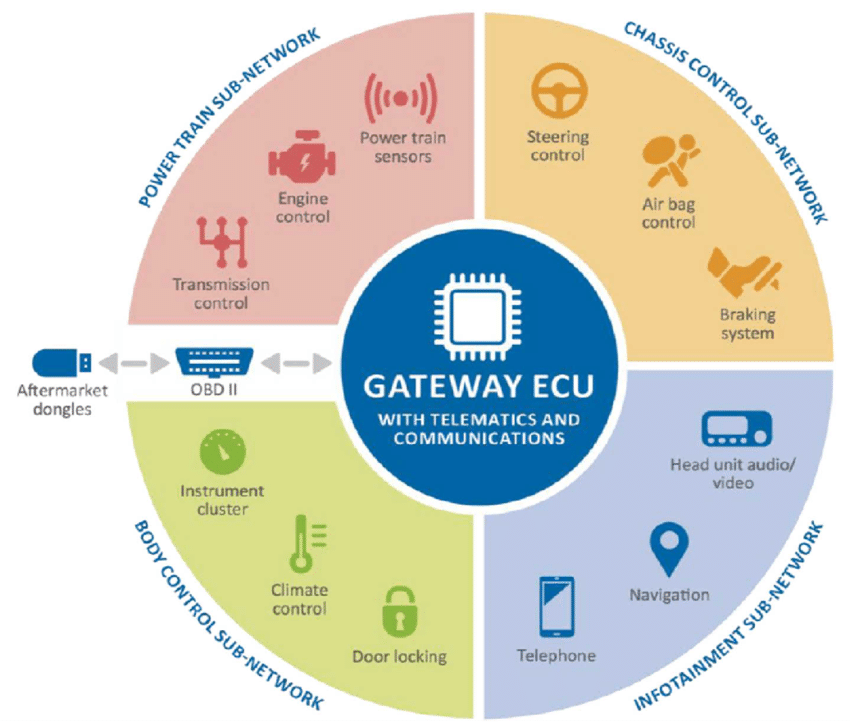
\includegraphics[width=\textwidth]{enisa.png}
	\caption{Typical intra vehicle network infrastructure \cite{Enisa}.}
    \label{fig:enisa}
\end{figure}
On top of their functional differences, these sub-networks often implement different network communications protocols. This means that there are multiple communication standards that are employed even within a single vehicle. The most common ones are: Controller Area Network (CAN), Local Interconnect Network (LIN), Media Oriented Systems Transport (MOST), FlexRay and LVDS \cite{Tuhoy}. Each of these protocols specifies how messages are exchanged within the appropriate sub-network. Their choice is based on the needs of a specific domain, as is illustrated in Table \ref{table:network_technologies} and \ref{table:network_technologies2}.
\begin{center}
\begin{table}[]
	\centering
	\begin{tabular}{|c|c|c|c|}
		\hline
		\rowcolor[HTML]{9B9B9B} 
		\textbf{Protocol} & \textbf{Bitrate} & \textbf{Medium} & \textbf{Protocol} \\ \hline
		LIN & 192 Kbps & Single Wire & Serial \\ \hline
		CAN & 1 Mbps & Twisted Pair & CSMA/CR \\ \hline
		FlexRay & 20 Mbps & Twister Pair/Optical Fibre & TDMA \\ \hline
		MOST &  150 Mbps & Optical Fibre & TDMA \\ \hline
		LVDS & 655 Mbps & Twisted Pair & Serial/parallel \\ \hline
	\end{tabular}
		\caption{An overview of different network technologies and their characteristics \cite{Tuhoy}.}
		\label{table:network_technologies}
\end{table}
\end{center}
\begin{table}[]
	\centering
	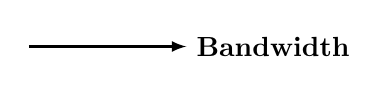
\begin{tikzpicture}[thick]
	\draw [black,  -latex] (0,6.5) -- (2,6.5) node [right] {\textbf{Bandwidth}} ;
	\end{tikzpicture}
	\begin{tabular}{cccccc}
		\cline{2-6}
		\multicolumn{1}{c|}{\textbf{LVDS}} & \multicolumn{1}{c|}{} & \multicolumn{1}{c|}{} & \multicolumn{1}{c|}{} & \multicolumn{1}{c|}{$\circ$} & \multicolumn{1}{c|}{$\circ$} \\ \cline{2-6} 
		\multicolumn{1}{c|}{\textbf{MOST}} & \multicolumn{1}{c|}{} & \multicolumn{1}{c|}{} & \multicolumn{1}{c|}{} & \multicolumn{1}{c|}{$\circ$} & \multicolumn{1}{c|}{} \\ \cline{2-6} 
		\multicolumn{1}{c|}{\textbf{FlexRay}} & \multicolumn{1}{c|}{} & \multicolumn{1}{c|}{$\circ$} & \multicolumn{1}{c|}{$\circ$} & \multicolumn{1}{c|}{} & \multicolumn{1}{c|}{} \\ \cline{2-6} 
		\multicolumn{1}{c|}{\textbf{CAN}} & \multicolumn{1}{c|}{$\circ$} & \multicolumn{1}{c|}{$\circ$} & \multicolumn{1}{c|}{$\circ$} & \multicolumn{1}{c|}{} & \multicolumn{1}{c|}{} \\ \cline{2-6} 
		\multicolumn{1}{c|}{\textbf{LIN}} & \multicolumn{1}{c|}{$\circ$} & \multicolumn{1}{c|}{} & \multicolumn{1}{c|}{} & \multicolumn{1}{c|}{} & \multicolumn{1}{c|}{} \\ \cline{2-6}
		& \textbf{Low} & \textbf{Real} &  &  & \textbf{Driver} \\
		& \textbf{Bandwith} & \textbf{Time} & \textbf{Safety} & \textbf{Infotainment} & \textbf{Assist} \\  
		& \textbf{Control} & \textbf{Control} & \textbf{Data} &  & \textbf{Cameras}         
	\end{tabular}
	\newline
	\caption{Mapping of traffic types to network technologies \cite{Tuhoy}.}
	\label{table:network_technologies2}
\end{table}
A critical component in vehicle networks is the gateway ECU. This component performs a frame or signal mapping function between two communication systems; allowing ECU's on different sub-networks, using distinct communication protocols, to exchange messages nonetheless. 
On top of acting as an intermediate between the different sub-networks of the vehicle, the gateway also acts as an entry point for OBD-II messages. Any message sent via the OBD-II port will be translated and forwarded by the gateway to the appropriate sub-network. It should come as no surprise that this component plays a crucial role when access control is introduced to the OBD-II interface.

\paragraph{Example: ABS}
Let's take a closer look at ABS to get a sense of how the intra vehicle network operates. ABS was designed to keep the wheels from locking up during braking. It consists of three main components: wheel speed sensors, a pump and a controller. Here's how it works \cite{wiki:ABS}:

\begin{itemize}
	\item The controller monitors the wheel speed sensors constantly (So each speed sensor periodically sends a message to the controller).
	
	\item The controller will recognize a wheel locking whenever it detects a rapid deceleration.
	
	\item Whenever the controller does detect a wheel locking up, it will use the pump (again by sending a message over the network) to regulate the pressure on the brake of that particular wheel, thereby keeping it from locking up.
\end{itemize}

\subsection{CAN}
\label{sec:can}

The CAN protocol has become a ubiquitous part of the automotive industry. In the context of internal vehicle networks, CAN messages have multiple purposes: First, there are informative messages, that are designed to transmit data from and to ECU's (e.g. the Anti-Lock System (ABS) broadcasting the speed of each wheel). Second, there are action messages that are designed to request another ECU to perform a specific action (e.g. the adaptive Cruise Control (ACC) module submitting a request for the brakes to be applied). Third, there are the diagnostic messages defined by the OBD-II protocol \cite{MillerB}. Naturally the last type of message is the focus of this paper. The following paragraphs are dedicated to the CAN protocol.

\subsubsection{Brief History} 
\label{subsec:can:briefhistory}

The history of CAN starts in 1983, when a couple of engineers at Bosch (soon aided by other engineers from Mercedes-Benz and Intel) start developing a new serial bus system for use in the automobile industry. It was not long before CAN was officially introduced at the SAE congress in Detroit as: 'Automotive Serial Controller Area Network'. The main characteristics of this new protocol were \cite{CANhistory}: 
\begin{itemize}
	\item An arbitration method that allows bus access to the message with the highest priority without delays.
	\item No need for a master node that is in charge of the bus.
	\item The identifier (ID) of these message identifies their content, not their destination or origin.
	\item This ID also determines the priority of the message within the network.
\end{itemize}
It didn't take long before the first CAN controller chips were developed in 1987 (by Intel and Philips respectively). The first official CAN specifications were standardised in the 90's, effectively paving the way for the CAN protocol to become an industry staple. To this day Bosh has been making sure that all CAN chips comply with their proposed standards, in an effort to avoid incompatible implementations. \footnote{For a comprehensive history of the CAN protocol see \cite{CANhistory}}

\subsubsection{Architecture}
\label{subsec:can:architecture}

A typical CAN network consists of a series of nodes connected by a two-wire bus. There are two physical CAN specifications: high speed CAN (see \cite{ISO11898-2}) and low speed (or fault tolerant) CAN (see \cite{ISO11898-3}). Every CAN node consists of:
\begin{itemize}
	\item CPU: This is effectively the 'brain' of the node, deciding what messages to send and taking the appropriate course of action whenever a message is received.
	\item Controller: in charge of reading and writing bits to and from the CAN bus.
	\item Transceiver: acts as in an intermediate between the bus and the controller, thereby translating between different signal levels.
\end{itemize}
This architecture specifies the minimum requirements of a CAN node. More often than not these nodes will also include a set of peripherals like sensors or actuators. It should be clear from this specification that this architecture applies to any common vehicle network (e.g. ECU's act as CAN nodes).

\subsubsection{CAN Frames}
\label{subsec:can:frames}
Since CAN is a message based protocol, it facilitates communication by transmitting short bursts of data called frames. There are four different types of CAN frames:
\begin{itemize}
	\item \textbf{Data frame:} used to transmit data with a specific identifier.
	\item \textbf{Remote frame:} used to request the transmission of data with a specific identifier.
	\item \textbf{Error frame:} transmitted whenever a node detects an error on the bus.
	\item \textbf{Overload frame:} transmitted by a node to include a delay between data or remote frame.
\end{itemize}
There are 2 frame formats: base frame format and the extended frame format. The only difference being that the extended frame format uses 29 identifier bits and the base frame format only uses 11. Table \ref{table:CANframeBase} and \ref{table:CANframeExtended} show the base and extended CAN frames respectively. The extended frame format is basically the same except for an additional identifier field (18 bits), immediately following the identifier extension bit (IDE) \cite{ISO11898-2,ISO11898-3}. 
\begin{table}[]
	\adjustbox{max width=\textwidth}{%
	\begin{tabular}{|c|c|c|c|c|c|c|c|c|}
		\hline
		\multirow{2}{*}{\textbf{SOF}} & \textbf{BASE} & \multirow{2}{*}{\textbf{RTR}} & \multirow{2}{*}{\textbf{IDE}} & \textbf{Control} & \multirow{2}{*}{\textbf{Data}} & \multirow{2}{*}{\textbf{CRC}} & \multirow{2}{*}{\textbf{ACK}} & \multirow{2}{*}{\textbf{EOF}} \\
		& \textbf{Identifier} & & & \textbf{Field} &  &  &  &  \\ \hline
		1 bit & 11 bits & 1 bit & 1 bit & 5 bits & 64 bits & 16 bits & 2 bits & 7 bits \\ \hline
	\end{tabular}
	}
	\caption{Base format CAN frame.}
	\label{table:CANframeBase}
\end{table}
\begin{table}
	\adjustbox{max width=\textwidth}{%
	\begin{tabular}{|c|c|c|c|c|c|c|c|c|c|c|}
		\hline
		\multirow{2}{*}{\textbf{SOF}} & \textbf{BASE} & \multirow{2}{*}{\textbf{SRR}} & \multirow{2}{*}{\textbf{IDE}} & \textbf{Ext.} & \multirow{2}{*}{\textbf{RTR}} & \textbf{Control} & \multirow{2}{*}{\textbf{Data}} & \multirow{2}{*}{\textbf{CRC}} & \multirow{2}{*}{\textbf{ACK}} & \multirow{2}{*}{\textbf{EOF}} \\
		& \textbf{ID} & & & \textbf{ID} & & \textbf{Field} &  &  & & \\ \hline
		1 bit & 11 bits & 1 bit & 1 bit & 18 bits & 1 bit & 6 bits & 64 bits & 16 bits & 2 bits & 7 bits \\ \hline
	\end{tabular}
	}
	\caption{Extended format CAN frame.}
	\label{table:CANframeExtended}	
\end{table}
\subsubsection{Data Transmission}
\label{subsec:can:data_transmission}

The operation of the CAN protocol is pretty straightforward: a node transmits a message with a specific ID on the bus. Any node connected to the same bus is able to receive the message, but only the nodes that are listening for this specific ID will take action. It is worth stressing again that the ID is used to identify the content, not the sender or receiver. As a matter of fact CAN does not provide any way of authenticating the sender or receiver, which results in various security related difficulties (see Section \ref{subsec:can:security_issues}). Aside from identifying the content, this ID is also used to solve the issue of message arbitration. CAN is a carrier sense multiple access protocol; each nodes observes the bus before transmitting data on it. If a node detects that the bus is in use, it waits for some time before trying again. However, this does not prevent multiple nodes from starting a data transfer at the same time. These situations were avoided with the introduction of bit wise message arbitration, which is discussed in the next section \cite{CANarbitration}.

\subsubsection{Message Arbitration}
\label{subsec:can:message_arbitration}

Whenever two or more nodes initiate a transmission on the bus at the same time, a bit wise message arbitration is performed. Every bit of the message ID can be either 1 or 0. The CAN specifications use the term dominant (logical 0) and recessive (logical 1). These terms originate from the fact that whenever more than one bit is simultaneously written to the bus, and one of these is dominant; the dominant bit 'wins', meaning a logical 0 will be seen on the bus. Whenever a node transmits a logical 1 but sees a logical 0; it realizes that there is a contention and re-queues its message for later transmission. Since the identifier is transmitted at the start of the CAN frame, the node with the numerically lowest identifier transmits more zeros at the start of the frame, and that is the node that wins the arbitration. Thus, messages with lower ID's have priority over messages with higher ID's. The decision to identify messages by their content (instead of their sender or receiver) is motivated by the fact that more important messages (e.g. errors) can be given a very low id, thereby ensuring they are prioritised \cite{ISO11898-2,ISO11898-3}. 

\subsubsection{Layering}
\label{subsec:can:layering}

It is common practice to decompose networking protocols into different abstract layers. This is done to simplify their design and make modularisation easier \cite{wiki:ProtocolStack}. In the case of the CAN protocol the layers are \cite{ISO11898-2,ISO11898-3}:

\begin{itemize}
	\item \textbf{Application layer:} OBD-II, CANOpen, etc.
	\item \textbf{Object layer:} message filtering and status handling.
	\item \textbf{Transfer layer:} error detection, message arbitration, bit timing, etc.
	\item \textbf{Physical layer:} signal voltages, pin-out configuration, etc.
\end{itemize}

\subsubsection{Security Issues}
\label{subsec:can:security_issues}

The CAN protocol has a number of inherent vulnerabilities that are common to any implementation. The most obvious and important ones are:

\begin{itemize}
	\item \textbf{Eavesdropping:} CAN frames are both physically and logically (no destination address) broadcasted on the network. This means that a malicious node on the bus can snoop on all communications; or even worse, send packets to any other node on the network \cite{Kosher}. 
	
	\item \textbf{No authentication:} CAN frames do not have source identifier fields, so there is no way for any node to be aware of the source of any messages it receives. This means that any compromised component (or any other form of unsanctioned access to the CAN bus for that matter) can inject arbitrary messages. The system has no way of knowing these messages were not sent by the appropriate component \cite{Kosher,CANissues}.
	
	\item \textbf{No encryption:} Speed and timing are deemed more important to the safety and performance of the vehicle than data security \cite{Klinedinst05}. A clear result of this is the decision to omit any encryption capabilities. This is because of the limited  computational power of ECU's, that makes it difficult to implement robust cryptographic algorithms \cite{CANissues}.  
	
	\item \textbf{Susceptibility to Denial of Service (DoS):} This problem arises mainly from the protocol's message arbitration method. Any malicious node can effectively spam the bus with high priority messages (only zeroes as ID), causing all other nodes to back off (no protection against "babbling idiots") \cite{Kosher,Pike15}.
	
	\item \textbf{Not Byzantine fault tolerant:} In most distributed systems, malicious attacks and software errors can cause a node to exhibit Byzantine (i.e. arbitrary) behaviour \cite{Byzantine}. Because of the distributed nature of any CAN system, there is imperfect information on whether a component has failed (or has been compromised by attack) or not. This could result in situations where the entire system fails, since a common consensus cannot be reached \cite{wiki:ByzantineFault}.\footnote{For more information on Byzantine faults, and how it is tolerated in a system see \cite{Byzantine} and \cite{wiki:ByzantineFault}.}
	
\end{itemize}
We refer te reader to \cite{ISO11898-2} and \cite{ISO11898-3} for more information on the CAN protocol.

\subsection{OBD-II}
\label{sec:obd}

\subsubsection{Brief History}
\label{subsec:obd:brief_history} 

There have been a lot of different proprietary automotive diagnostics systems introduced over the years, before a standard arrived with the introduction of OBD-II. This brief history, cited from \cite{OBDhistory}, does an excellent job of concisely explaining how OBD-II came to be:

\begin{displayquote}
	The origins of OBD-II actually date back to 1982 in California, when the California Air Resources Board (ARB) began developing regulations that would require all vehicles sold in that state starting in 1988 to have an onboard diagnostic system to detect emission failures. The original onboard diagnostic system (which has since become known as OBD-I) was relatively simple and only monitored the oxygen sensor, exhaust gas circulation system, fuel delivery system and engine control module.
	
	OBD-I was a step in the right direction, but lacked any requirement for standardization between different makes and models of vehicles. You still had to have different adapters to work on different vehicles, and some systems could only be accessed with costly "dealer" scan tools. So when ARB set about to develop standards for the current OBDII system, standardization was a priority: a standardized 16-pin data link connector (DLC) with specific pins assigned specific functions, standardized electronic protocols, standardized diagnostic trouble codes (DTCs), and standardized terminology.
	
	Another limitation of OBD-I was that it couldn't detect certain kinds of problems such as a dead catalytic converter or one that had been removed. Nor could it detect ignition misfires or evaporative emission problems. Furthermore, OBD-I systems would only illuminate the MIL light after a failure had occurred. It had no way of monitoring progressive deterioration of emissions-related components. So it became apparent that a more sophisticated system would be required. The California Air Resources Board eventually developed standards for the next generation OBD system, which were proposed in 1989 and became known as OBD-II. The new standards required a phase-in starting in 1994. The auto makers were given until the 1996 model year to complete the phase-in for their California vehicles.
	
	Similar standards were incorporated into the federal Clean Air Act in 1990 which also required all 49-state vehicles to be OBD-II equipped by 1996 -- with one loophole. The OBD-II systems would not have to be fully compliant until 1999. So some 1996 OBD-II systems may lack one of the features normally required to meet the OBD-II specs, such as the evaporative emissions purge test.
\end{displayquote}

\subsubsection{Design Goals} 
\label{subsec:obd:design_goal}

OBD-II is a specification that has been introduced to allow for self diagnostic and reporting functionality for ECU's inside a vehicle, and has been mandatory in every car produced in the united states since 1996 \cite{wiki:OBD}. It allows users (testers, developers, repairmen, etc.) to query ECU's about diagnostics information, in order to perform a detailed analysis of the vehicles internal systems. Specifically, the goals of OBD-II upon introduction were: 
\begin{itemize}
	\item Standardisation: information is communicated in a standardized format to allow for 1 tool to be used on many vehicles.
	\item Certification: Every vehicle manufacturer is required to apply for certification, which includes submitting a detailed description of how the OBD-II protocol was implemented.
	\item Help lowering emissions by identifying emission controls in need of repair.
\end{itemize} 
The system can also be very useful in a number of other situations: a repairman looking for a specific component that is to be repaired, an employee at the factory testing all components before the vehicle is ready to be sold, a policeman analysing a vehicle after a crash to determine what caused the accident, a software developer testing the operation of a newly developed ECU, etc. 

\subsubsection{DLC}
\label{subsec:obd:dlc}

To allow a user to communicate with the vehicle's internal network, OBD-II introduces the data link connector (DLC). The DLC is a 16-pin hardware interface (although only 9 pins are specified by the standard) that is generally found close to the steering wheel (by law it is required to be installed within 0.61 m of the steering wheel) \cite{wiki:OBD}. There are 2 basic types of connectors: Type A as seen in Figure \ref{fig:typeA} (using a 12V power supply) and Type B as seen in Figure \ref{fig:typeB} (using a 24V power supply). The design of the two connector types prevents the insertion of a type A male plug into a type B female socket.

\begin{figure}[h]
	\centering
	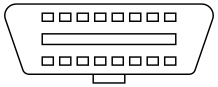
\includegraphics{typeA.png}
	\caption{Type A female connector \cite{wiki:OBD}.}
	\label{fig:typeA}
\end{figure}

\begin{figure}[h]
	\centering
	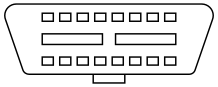
\includegraphics{typeB.png}
	\caption{Type B female connector \cite{wiki:OBD}.}
	\label{fig:typeB}
\end{figure}

\subsubsection{PID}
\label{subsec:obd:pid}

OBD-II introduces parameter ID's (PID), which are codes used to identify and query specific data. The protocol is designed to work with multiple signalling protocols (the messaging protocol that is used to request and receive data from the network), but the CAN protocol is mostly implemented (Since 2008 all new vehicles sold in the US implement this signalling protocol \cite{OBDconnector}). \newline
\newline
There are multiple ways for a user to interact with this interface:
\begin{itemize}
	\item A standard diagnostic scanning tool, which is a dedicated device that consists of a small hand-held module (equipped with a small screen and some buttons), connected to a male DLC (The DLC inside the vehicle is always female).
	
	\item An advanced Diagnostic scanning tool that includes a DLC-connector with wifi/Bluetooth compatibility, allowing for remote diagnostics via smartphone or PC.
	
	\item A DLC-connector with a USB adapter, allowing access via dedicated software on a PC. Since 2014, all new cars in the US support the SAE J2534 "PassThru" standard, which is a Windows application programming interface (API) that provides a standard way to communicate with a car's internal buses \cite{Kosher}.\footnote{For more information on SAE J2534, see the full API reference at: \url{https://tunertools.com/prodimages/DrewTech/Manuals/PassThru\textunderscore API-1.pdf}}
	
	\item A data logger, which is designed to capture real-time data while the vehicle is in operation.
\end{itemize}
Typically, ODB-II is used like this (CAN as signalling protocol): First, the user enters the PID of the data (s)he wants to query into a diagnostic tool. Second, this data is packaged in a CAN frame and sent over the CAN-bus. Third, the ECU that is responsible for the data identified by the PID in the message recognizes it as it's own, and transmits a CAN frame containing the requested data. Fourth, the diagnostic tool recognizes the response and displays the data to the user \cite{wiki:PID}. The OBD-II port can also be used to upgrade the ECU's firmware or to perform a myriad of other diagnostic tasks.

\subsubsection{Security Issues}
\label{subsec:obd:security_issues}

It is a well-known fact that the automotive industry has always considered safety a critical engineering concern \cite{Dyer}. Unfortunately, it is unclear whether developers (especially concerning the internal network) have considered the security in their design. It seems this is not the case because of three reasons. First, as is asserted in \cite{MillerB}, 'there is no inherent support for addressing, encryption or authentication'. Second, most of the networks and ECU's were designed when access to the bus required physical access to the vehicle, therefore security was not a primary concern. Third, speed and timing are considered more important to the safety of the vehicle than the security of transmitted data \cite{Klinedinst05}. This vulnerability is worsened by the fact that the attack surface of modern automobiles is growing swiftly, as more sophisticated services and communications features are incorporated into vehicles \cite{Kosher}. The OBD-II specification is one of these, since its interface provides direct access to the internal vehicle network. This allows malicious agents to easily construct and insert CAN messages to alter the vehicle's behaviour, as has been frequently demonstrated by Charlie Miller and Chris Valasek's exploits \cite{MillerA, MillerB, MillerC}. The goal of this research paper is to design a solution that prevents malicious agents from mounting attacks via the OBD-II interface, while still allowing for the system to function properly (i.e. performing diagnostics and maintenance). 

\section{Preliminaries}
\label{chap:preliminaries}

This section serves as a technical primer to all the security related software solutions that are employed in this paper. The reader should keep in mind that the selection of algorithms and systems presented here is far from comprehensive; only those that are relevant to the solution presented in this paper are discussed.

\subsection{ECU Microcontrollers}
\label{sec:microcontrollers}

An ECU is an embedded computer that is designed to perform a specific function. The core of any ECU is a small computer on an integrated circuit called a microcontroller. A microcontroller consists of one or more central processing units (CPU) along with memory and programmable input/output peripherals. There a couple of characteristics of microcontrollers that are touched upon in the course of this paper, so a description of these is given next:

\begin{itemize}
	\item \textbf{Word size:} The word size of a microcontroller (or any computer for that matter) is the natural unit of data used by a particular processor. A word is a fixed-sized piece of data handled as a single unit by the instruction set or the hardware of the processor. The number of bits in a word is an important characteristic of any microcontroller. Within the context of ECU's, word sizes of 8 bits (e.g. driver information), 16 bits (e.g. vehicle control) and 32 bits (e.g. power train) are most common \cite{ECU}.
	
	\item \textbf{Clock rate:} The clock rate of a CPU refers to the rate at which it processes words of data. it is used as an indicator of the processor's speed. It is measured in clock cycles per second or hertz (Hz). 
	
	\item \textbf{Memory:} There are two basic types of memory: 
	\begin{itemize}
		\item \textbf{Data Memory}: Data memory is where variables and all intermediate calculations are stored by the CPU. It is generally implemented by RAM\footnote{random access memory (RAM) is a type of memory where individual data can be read or written in almost the same amount of time irrespective of the physical location of data inside the memory.}. This data is often volatile, meaning the data is lost when power is removed.
		
		\item \textbf{Program memory}: Program memory is where the application is stored, i.e. the code itself. This type of memory is implemented using non-volatile storage technologies like ROM \footnote{Read-only memory (ROM) is a type of non-volatile memory where the data stored can not be modified (or where it is considered very difficult to do so).}, EPROM\footnote{erasable programmable read-only memory (EPROM) is a non-volatile type of memory that can be erased (by exposing the chip the ultraviolet light) and reprogrammed.}, EEPROM\footnote{Electrically erasable programmable read-only Memory (EEPROM) is a type of non-volatile memory that can be erased and reprogrammed electronically.} or Flash Memory\footnote{Flash memory is type of EEPROM  that can be electrically erased and reprogrammed much faster than regular EEPROM chips by using large erase blocks.}.
	\end{itemize}
	
	\item \textbf{Serial Communications Interfaces:} Serial communications is a way of communication in computer networks where bits are transmitted one bit at a time (e.g. CAN). This is in contrast to parallel communications where a link is used with several parallel channels, allowing multiple bits to be sent at the same time (e.g. USB). Most microcontrollers offer dedicated hardware allowing for easy communication with other devices (e.g. CAN controller).
	
	\item \textbf{Others:} Most microcontrollers offer various other hardware like: a timer, an analog-to-digital convertor (ADC) that allows for an analog signal (like the output of a sensor) to be transformed into a digital signal, a clock generator, etc.
\end{itemize}

\subsection{Role-Base Access Control}
\label{sec:RBAC}

Role-based access control (RBAC) is a well-defined way of restricting system access to authorized users. It especially useful in large enterprises where roles are created for various job functions. Each role is assigned the necessary permissions to interact with a secured system (e.g. the company database, the local private network, development software, etc). The idea is that a worker is assigned a role based on what (s)he requires to do their job, and nothing more. To avoid that workers are granted permissions they do not need. There are two basic types of RBAC \cite{wiki:RBAC}.

\begin{itemize}
	\item \textbf{Mandatory Access Control:} In a system where mandatory access control (MAC) is a enforced, only the administrator of the system is able to create and assign roles. This is done by defining a security policy that users are unable to override or alter. The administrator of the system is called the security policy administrator.
	
	\item \textbf{Discretionary Access Control:} When discretionary access control (DAC) is enforced, it is up to the users themselves to make policy decisions and/or assign security attributes.
\end{itemize}

\subsubsection{Permission Table}
\label{subsec:permissions_table}

RBAC systems are generally implemented by introducing a permission table. This table is a software representation of the agreed-upon security policy. There is an entry in this table for each permission that can be assigned (e.g. access to files, permission to create/delete folders, etc). Every field of each entry corresponds with a role, and whether this role is granted the corresponding permission. 

\subsection{Public Key Cryptography}
\label{sec:PKC}

\subsubsection{Cryptography} 
\label{subsec:cryptography}

The primary goal of cryptography in general is to allow for secure communication between two parties. This means that protocols are designed that prevent third parties or the public in general from reading private messages. This is done by encrypting the message, which consists of converting the information from a readable state to apparent nonsense. Only the intended recipient should be able to restore the information to it's original form, which is called decryption. To allow for this to work, the procedure of encryption and decryption should only be possible by the sender and the receiver respectively. Generally this procedure consists of two parts. First, there is the cypher, which is the algorithm that does the actual conversion. Second, there's the secret key, which is used by the cipher together with the input (plaintext) to create the encrypted output (ciphertext). The main advantage of this architecture is that the chosen cipher can be made public, as long as the key is kept secret. The receiver of the secret message, who is in possession of the same secret key, runs the same cipher in reverse with the secret key and the ciphertext as inputs, yielding the original plaintext \cite{wiki:Cryptography}.

\subsubsection{Symmetric vs Asymmetric}
\label{subsec:symmetric_vs_assymetric}

The procedure outlined above is called symmetric key cryptography, since both parties are in possession of the same secret key. The disadvantage here is that these keys need to be securely exchanged beforehand (e.g. via a secure channel) to allow for secure communications. Asymmetric (or public key) cryptography offers a solution to this problem. In this case, a key pair is created where each one serves a specific function. The first one is called the private key, which is meant to be kept secret at all times by the owner. The second one is called the public key, which is disseminated widely to the public. The idea is that if someone wants to send an encrypted message to the owner of the private key, (s)he looks up the corresponding public key (generally found online); uses the public key to encrypt a message, and sends this message to the owner. Since only the owner is in possession of the corresponding private key, only (s)he is able to decrypt the message.

\subsection{Key Exchange} 
\label{sec:key_exchange}

The specifications of symmetric and asymmetric encryption are sound. However they both rely on both parties being in possession of the right key. In the case of asymmetric encryption this is easy: The owner generates a new public/private key pair, stores the private key in a safe location, and distributes the corresponding public key on the Internet. Anyone who wants to securely communicate with the owner only has to look up the corresponding public key. This procedure does not apply to symmetric encryption however, since only the sender and receiver should be in possession of the secret key. One way of safely distributing the key is to use a secure communications channel. Examples of this are: a text message, a phone call, physically handing over the key, sending a letter, etc. However, it is clear that in most situations this method simply will not do, since it requires significant effort before a secure communication session can be established. Two more realistic alternatives exist: using asymmetric keys to establish a session key and key exchange algorithms. Both will be discussed in turn next.

\subsubsection{Session Keys} 
\label{subsec:session_keys}

The free distribution of public keys can be leveraged to establish a new temporary shared key, also called a session key. If Alice has an asymmetric key pair already established, and Bob wishes to establish a shared secret key with Alice; bob only has to look up Alice's public key, generate a new session key, encrypt the new session key using Bob's public key, and send it to Alice. Alice can then decrypt the session key using her private key. In the end both parties are in possession of the new session key, and a secure communication can be established. Now, the reader might wonder why it is necessary to establish a session key, since secure communications could also be performed using asymmetric keys (granted they both have an asymmetric key pair). This is mainly due to performance. Asymmetric encryption requires significantly longer keys to guarantee the same level of security, and the corresponding procedures (e.g. encryption, decryption, signing, etc.) take significantly longer to perform. Therefore, it is often beneficial to establish a session key, instead of repeatedly using asymmetric keys.

\subsubsection{Key Exchange Algorithms} 
\label{subsec:key_exhange_algorithms}

Key exchange algorithms allow two parties that have no prior knowledge of each other to establish a shared secret key over an insecure channel. The most famous example of such an algorithm is the Diffie-Hellman key exchange method \footnote{for more information on Diffie-Hellman see \cite{wiki:DH}}. These algorithms typically rely on computationally hard to solve mathematical problems such as the discrete logarithm.

\subsection{Authentication} 
\label{sec:authentication}

Besides protecting messages from being read by a third party, the recipient of the message might also want certainty on who sent it in the first place, as well as knowing that the message has not been tampered with. In other words the recipient wants to guarantee the integrity of the message, on top of authenticating the sender. Fortunately asymmetric and symmetric cryptography offer solutions in the form of digital signatures and message authentication codes respectively. Before going into this however, it is necessary to first take a look at hash functions.

\subsubsection{Hash functions} 
\label{subsec:hash_functions}

A hash function is used to map data of arbitrary size to data of a fixed size. The values returned by a hash function are called hash values, hash codes, digests, or simply hashes. For a hash function to be useful in cryptography (also called a cryptographic hash function) it has to possess the following properties \cite{wiki:Hash}:

\begin{itemize}
	\item The same message always results in the same hash value.
	\item The hash function does not take long to perform.
	\item It is infeasible to reconstruct the original message from the hash value.
	\item Two similar messages have widely varying hash values.
	\item it is infeasible to find two different messages with the same hash value.
\end{itemize}

\subsubsection{Digital Signatures} 
\label{subsec:digital_signature}

A digital signature is used to verify the authenticity of digital messages. The principle is simple: If Alice wants to send an authenticated message to Bob, she will first sign the message using her private key. She then sends the message together with the generated signature to Bob. Bob can then check the authenticity of the message by verifying the signature using Alice's public key. If the verification was successful, Bob can safely assume 2 things: the message was sent by Alice (since she is in possession of the corresponding private key) and the message was not tampered with in transit (since in that case the signature would no longer match the message, resulting in a failed verification). Two additional algorithms are required: a signing algorithm and a signature verification algorithm. Ideally the signing algorithm would produce a signature of the same size, regardless of the size of the original message. This is where cryptographic hash functions come in, since they possess this property. Generally the message will first be hashed to a fixed size, before being processed by the signing algorithm. Besides guaranteeing a fixed sized output, this also improves the overall efficiency \cite{wiki:DigitalSignature}.

\subsubsection{MAC's} 
\label{subsec:MAC}
a message authentication code (MAC) serves the same function as a digital signature algorithm. Namely, guaranteeing the authenticity and integrity of a transmitted message. The main difference is that MAC's are based on symmetric keys rather than asymmetric keys. 

\subsection{Authenticated Key Agreement}
\label{sec:AK}

As will become apparent in Section \ref{subsec:authenticated_key_agreement_procedure}, it is generally advised to combine authentication and shared secret establishment into a single procedure. This is called authenticated key agreement (AK). In AK systems both parties are mutually authenticated while a shared secret is established. It is only assured that both parties are able to generate the shared secret, not that this secret was actually computed. A protocol that also guarantee to both parties that the other party actually computed the secret is called authenticated key agreement with key confirmation (AKC) \cite{Blake-Wilson}.

\subsection{Security Level}
\label{sec:security_level}

The security level of a cryptographic primitive (e.g. a hash function, a key, a cipher) refers to the difficulty for any attacker to break it. The security level is usually expressed in bits, where  an $n$-bit security level indicates that an attacker would have to perform (at least) $2^n$ operations to effectively crack the cryptographic primitive. It is very useful when comparing between different cryptographic algorithms, which will be done frequently during the course of this paper.

\section{Chosen Security Systems}
Previously an attempt was made to explain the basic principles behind the security systems that will be implemented in this paper. A multitude of various approaches to these systems exist however. The difference between them is mostly down to the mathematical structure of the approach, as well as the effect this has on efficiency and performance when they are implemented. This section will give an overview of the different implementations that were chosen for this paper, as well as motivating why these decisions were made.

\subsection{Elliptic Curve Cryptography}
\label{subsec:ECC}

There exist a couple of well-known public key cryptography technologies. The basic principle behind all of them is the use of functions that are easy to perform in one direction, but where the inverse is far more difficult (these are called trapdoor functions). Take prime multiplication for example: if we take two prime numbers $p$ and $q$, it is quite easy to calculate the product $n=pq$. However the factorisation of $n$ into $p$ and $q$ is way more difficult, especially when these numbers are significantly large. This is called the factoring problem and is the backbone of the Rivest Shamir Adleman (RSA) cryptosystem. This property is then leveraged to make it difficult to calculate the private key from the public key, while calculating the public key from a random private key is rendered trivial. The problem with RSA however is that it requires very long key sizes (currently the minimal recommended key size is 2048 bits \cite{RSAlength}), and the corresponding procedures are very slow \cite{wiki:RSA}. This wouldn't be a problem if the enough processing capacity were available. However, for the typical microcontroller found in ECU's this is not the case. It was shown in \cite{Sethi} that using the RSA digital signature operation (with a key size of 2048 bit) in a typical 8-bit microcontroller (the ATmega328, which has a clock speed of 16 MHz, 2 kB of RAM, and 32 kB of flash memory), takes roughly 26 minutes to complete. Luckily elliptic curve cryptography offers a solution to this.

\paragraph{ECC} Elliptic curve cryptography (ECC) is an approach to public-key cryptography based on the algebraic structure of elliptic curves over finite fields instead of plain Galois fields, like most other non-EC based algorithms. Where RSA was based on the difficulty of the factorisation problem, ECC is based on the discrete logarithm of a random elliptic curve element with respect to a publicly known base point, which is called the elliptic curve discrete logarithm problem (ECDLP) \cite{Siddiqui}. The advantage of ECDLP is that it is way more difficult to solve than the factorisation problem of RSA. This means that for the same key size, ECC is more secure than RSA (i.e. assures a greater security level). In other words, when using ECC we can use smaller key sizes, while still guaranteeing the same level of security. Running the elliptic curve digital signature algorithm (ECDSA) on the same microcontroller as before, with a curve that guarantees the same level of safety as an RSA 2048 bit key, takes roughly 6 seconds to complete. This is a significant improvement over the 26 minutes it took RSA \cite{Sethi}.

\subsubsection{ECDSA} 
\label{subsubsec:ecdsa}

The elliptic curve digital signature algorithm (ECDSA) is the default elliptic curve variant of digital signatures. 

\subsubsection{ECDH} 
\label{subsubsec:ecdh}

Besides using ECC for digital signatures with ECDSA, another ECC based protocol that is chosen in this paper is elliptic curve Diffie-Hellman (ECDH). Like normal Diffie-Hellman it is used when two communicating parties wish to establish a shared secret (or session key) over an insecure channel. First, the two communication parties agree on the elliptic curve they will use. Second, they both generate an ECC key pair. Third, they exchange their public keys. In the last step they both use their own private key, together with the public key they received to generate the same secret value. Any third party listening on the channel only knows both public keys, which is not enough to easily calculate the shared secret since they would have to solve the ECDLP.

\subsubsection{ECDHE\_ECDSA} 
\label{subsubsec:ecdh_ecdsa}

As mentioned in Section \ref{sec:AK} and illustrated in Section \ref{subsec:authenticated_key_agreement_procedure}, it is a common practice to combine authentication and shared secret establishment into a single procedure. In \cite{RFC4492} multiple methods are proposed that perform ECDH, while also providing authentication using elliptic curve digital signatures. One of these methods is called ECDHE\_ECDSA and is illustrated in Figure \ref{fig:ECDH2}. The extra E in ECDHE comes from th fact that this procedure uses "ephemeral" (i.e temporary) keys. Two communicating parties (Alice and Bob) are both in possession of an elliptic curve private/public key pair: $Pb_a$,$Pr_a$ (Alice) and $Pb_b$,$Pr_b$ (Bob). Alice signals to Bob that she wishes to initiate a ECDHE\_ECDSA sequence by sending a 'hello' message to Bob. Bob then creates a new ephemeral elliptic curve key pair: $Pb_{bE}$,$Pr_{bE}$, signs the new ephemeral public key using his own private key: Sig($Pb_{bE}$,$Pr_b$), and sends this to Alice. She will first verify the signature: Ver(Sig,$Pb_{b}$), thus authenticating Bob to Alice. After which she will also generate her own ephemeral key pair using the same curve as Bob: KGen($Pb_{aE}$,$Pr_{aE}$), before signing the new public key and sending it to Bob: Sig($Pb_{aE}$,$Pr_a$). Bob will then in turn verify the signature using Alice's public key: Ver(Sig,$Pb_{a}$). Alice and Bob are now both in possession of each other's ephemeral public keys, to use ECDH to generate a shared secret: $K$=ECDH($Pr_{aE}$,$Pb_{bE}$) for Alice and $K$=ECDH($Pr_{bE}$,$Pb_{aE}$) for Bob. The attentive reader might wonder why these ephemeral key pairs are generated at all. why not use the pre-existing key pairs $Pb_a$,$Pr_a$ and $Pb_b$,$Pr_b$ to generate the shared secret. This is because introducing these ephemeral keys guarantees perfect forward secrecy (PFS)\footnote{Perfect forward secrecy is guaranteed when a posteriori leak of one of the used private keys (e.g. $Pr_a$ and $Pr_b$ in figure \ref{fig:ECDH2}) does not result in the communication session (i.e. the session key) being compromised.}.


\begin{figure}[h]
	\centering
	\fbox{
		\procedure{ECDHE\_ECDSA}{%
			\textbf{Alice}  \<\< \textbf{Bob} \\
			\text{$Pb_a$,$Pr_a$} \<\< \text{$Pb_b$,$Pr_b$} \\
			\< \sendmessageright{top=\text{hello}} \<\\
			\<\< \text{KGen($Pb_{bE}$,$Pr_{bE}$)} \\
			\< \sendmessageleft{top=\text{Sig($Pb_{bE}$,$Pr_b$)}} \<\\
			\text{Ver(Sig,$Pb_{b}$)} \<\< \\
			\text{KGen($Pb_{aE}$,$Pr_{aE}$)} \<\< \\
			\< \sendmessageright{top=\text{Sig($Pb_{aE}$,$Pr_a$)}} \<\\
			\<\< \text{Ver(Sig,$Pb_{a}$)} \\
			\text{$K$=ECDH($Pr_{aE}$,$Pb_{bE}$)} \<\< \text{$K$=ECDH($Pr_{bE}$,$Pb_{aE}$)} \\
		}
	}
	\caption{ECDHE\_ECDSA}
	\label{fig:ECDH2}
\end{figure} 

\subsection{SHA-256 and SHA-512} 
\label{subsec:sha}

A lot of cryptographic procedures require the data to be hashed first; the implementation of this research paper is certainly no exception. The choice was made to use the secure hash algorithm (SHA) family of hash functions. SHA constitutes a large set of cryptographic hash functions that were designed by the United States National Security Institute (NSA). There exist four distinct sets of SHA \cite{wiki:SHA}:

\begin{itemize}
	\item \textbf{SHA-0}: Published in 1993, was withdrawn shortly after publication because of a significant flaw.
	
	\item \textbf{SHA-1}: Published in 1995 as a replacement to SHA-0. It has been considered insufficiently secure since 2011 \cite{Stevens}.
	
	\item \textbf{SHA-2}: Published in 2001, consists of six hash functions with hash values that are 224, 256, 384 or 512 bits in size: SHA-224, SHA-256, SHA-384, SHA-512, SHA-512/224 and SHA-512/256 \cite{RFC6234}.
	
	\item \textbf{SHA-3}: Pubished in 2015, subset of the broader cryptographic primitive family Keccak, conists of the following hash functions: SHA3-224, SHA3-256, SHA3-384 and SHA3-512 \cite{SHA3}.
\end{itemize} 
While the SHA-3 hash functions were an obvious candidate, simply because they are newer and deemed more secure, the choice was made to work with the SHA-2 hash functions instead. This is because SHA-2 libraries are better when it comes to performance \cite{Murvay}.

\subsection{HMAC} 
\label{subsec:hmac}

Once a session key is established between two parties this can be used to authenticate the messages they send to each other. Since this configuration is symmetric, i.e. they both share the same secret, this is done by using a message authentication code (MAC). The choice was made to work with a hash-based message authentication code (HMAC). HMAC is a specific type of message authentication code (MAC) that uses a cryptographic hash function as well as a secret cryptographic key (in our case the session key established using ECDH). More specifically, HMAC-256 (HMAC using SHA-256) was used since it is sufficiently secure, as well as being efficient in terms of performance and memory footprint.

